\chapter{Experimentación }
\section{Técnica 1:Base de datos basado en Neo4j}
\subsection{Creación de la Base de datos}
Creamos los scripts de inicialización de la base de datos de películas.
Para esto en la Figura \ref{fig:info} vemos las característicasa de nuestra base de datos, desde los tipos de nodos y las relaciones hasta las propiedades que tienen cada nodo.
\begin{figure}[H]
    \centering
    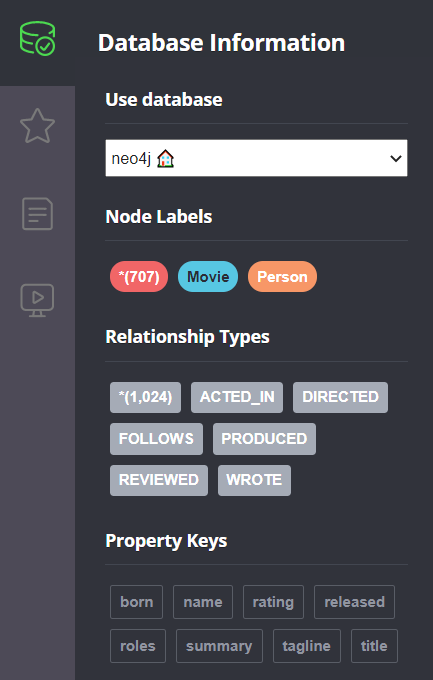
\includegraphics[scale=0.45]{Graficos/info.png}
    \caption{Datos generales de la base de datos de películas}
    \label{fig:info}
\end{figure}
A continuación en la Figura \ref{fig:graph_1} muestra el grafo del pequeño segmento tomado para la muestra de nodo y relaciones correspondientes.
\begin{figure}[H]
    \centering
    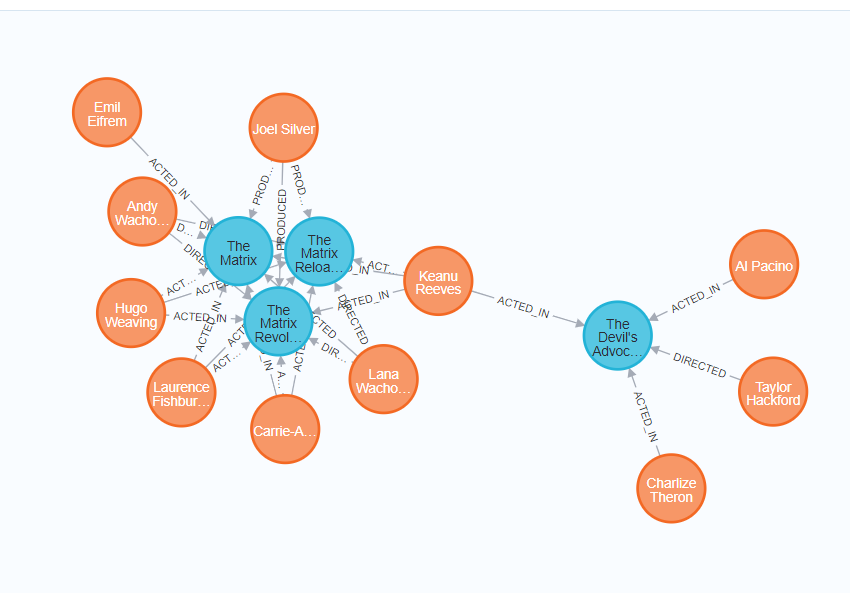
\includegraphics[scale=0.6]{Graficos/graph1.png}
    \caption{Gráfo de retorno según el tipo de nodo n como un pequeño segmento de toda la base de datos de películas}
    \label{fig:graph_1}
\end{figure}
Para nuestro segundo tipo de nodo tenemos como tag a película en el cual la Figura \ref{fig:tab_2} muestra un pequeño fragmento en forma de tabla de los nodos película y sus respectivos atributos:
\begin{itemize}
    \item Tagline: Frase representativa de dicha película.
    \item Title: Nombre de la película y el año en el que fue lanzada.
\end{itemize}
Después, es mostrado en forma de nodos de grafo las películas que ingresamos a nuestra base de datos en la Figura \ref{fig:graph_2}
\begin{figure}[H]
    \centering
    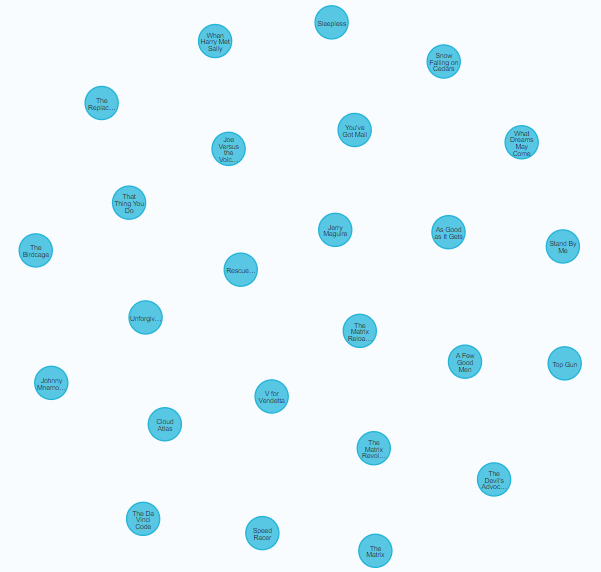
\includegraphics[scale=0.8]{Graficos/graph2.png}
    \caption{Grafo de nodos de películas sin relaciones ni conexiones.}
    \label{fig:graph_2}
\end{figure}
\begin{figure}[H]
    \centering
    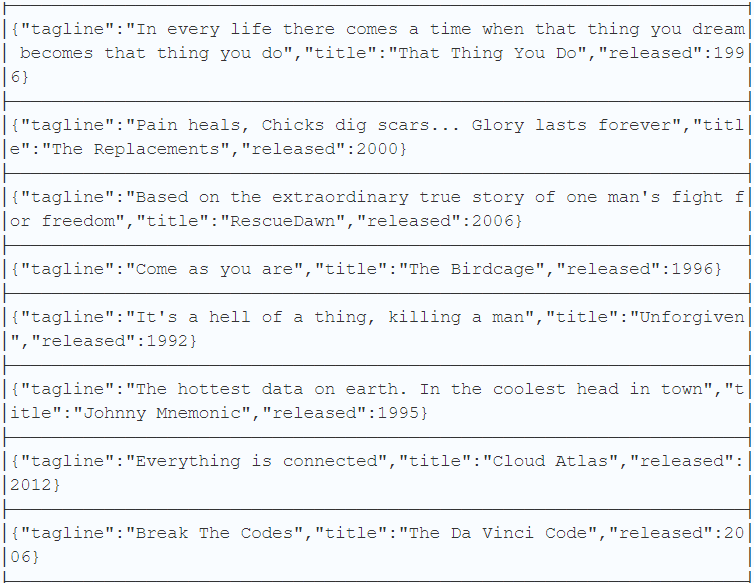
\includegraphics[scale=0.7]{Graficos/tabla2.png}
    \caption{Tabla de los nodos película de la base de datos}
    \label{fig:tab_2}
\end{figure}
Finalmente mostramos el tercer tipo de nodo de nuestra base de datos de películas el cual tiene de etiqueta person , el cual brinda los datos y atributos como muestra en la Figura \ref{fig:tab_3} que representan:
\begin{itemize}
    \item Actores.
    \item Escritores.
    \item Directores.
    \item Productores.
\end{itemize}
Y de manera general la Figura \ref{fig:tab_3} muestra como nodos sin conexiones ni relaciones los nodos person que existen en nuestra base de datos
\begin{figure}[H]
    \centering
    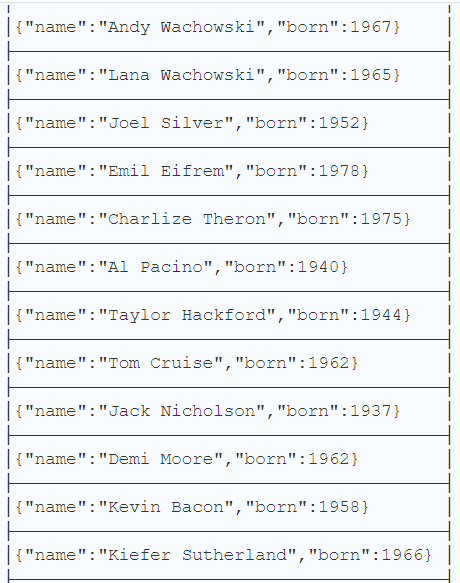
\includegraphics[scale=0.7]{Graficos/tab3.png}
    \caption{Tabla de los nodos person de la base de datos}
    \label{fig:tab_3}
\end{figure}
\begin{figure}[H]
    \centering
    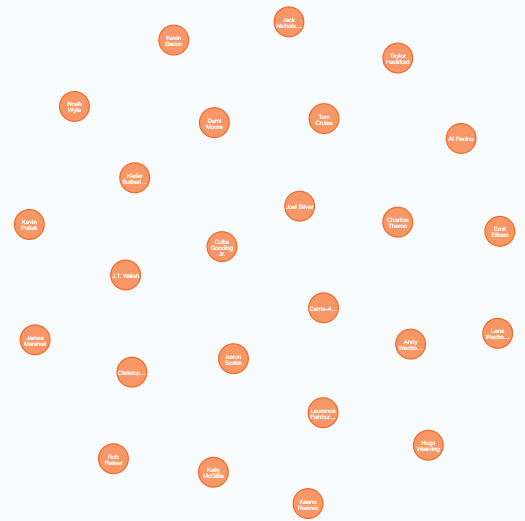
\includegraphics[scale=0.8]{Graficos/graph3.png}
    \caption{Nodos grafo con la etiqueta person de la base de datos de películas}
    \label{fig:graph_3}
\end{figure}
\subsection{Análisis de la base de datos}
\subsubsection{Consulta de los atributos de un nodo}
El objetivo es mostrar como se realizan para mostrar un nodo en concreto usando los comandos de consulta del lenguaje Cypher.\\
En la Figura \ref{fig:match_1} vemos en la sintaxis de escritura que se usa MATCH para referirse a un conjunto de nodos de un tipo representado por una variable el cual con LIMIT definimos la cantidad de nodos a mostrar.\\
En la Figura \ref{fig:match_2} notamos que ya explicitamente escogemos el nodo de una película buscandola por el título de esta para mostrar el título y el año en el que fue realizado dicha película.
\begin{itemize}
    \item Mostrar todos los nodos de un tipo en concreto , ya sea persona o película.
    \begin{figure}[H]
    \centering
    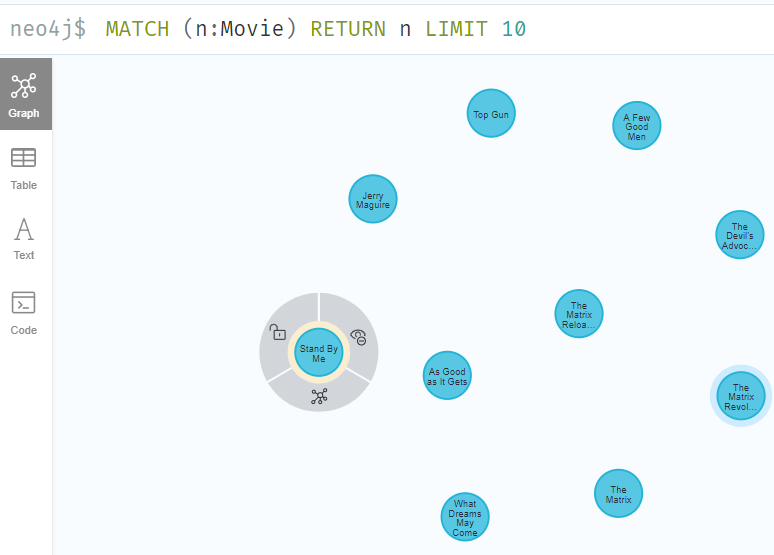
\includegraphics[scale=0.6]{Graficos/match1.png}
    \caption{Nodos película mostrados en grafo limitado a 10}
    \label{fig:match_1}
    \end{figure}
    \begin{figure}[H]
    \centering
    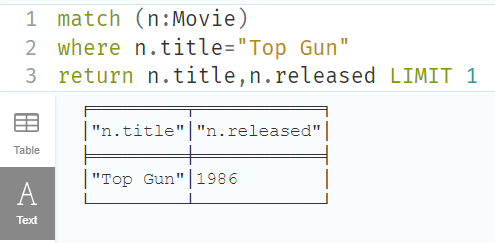
\includegraphics[scale=0.85]{Graficos/match2.png}
    \caption{Nodo película con titulo de Top Gun y su año en el que fue realizado}
    \label{fig:match_2}
    \end{figure}
    \item Mostrar un nodo y sus atributos en concreto
    En la Figura \ref{fig:att} vemos como un nodo película muestra sus relaciones con otros nodos en forma gráfica.
    \begin{figure}[H]
    \centering
    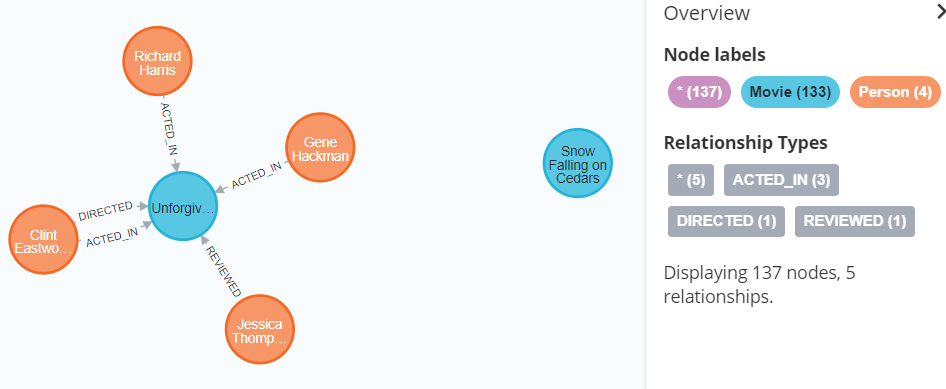
\includegraphics[scale=0.5]{Graficos/att.png}
    \caption{Nodo película Unforgiven con sus respectivas relaciones}
    \label{fig:att}
    \end{figure}
\end{itemize}
\subsubsection{Consulta encapsulada por diversos atributos}
En la Figura \ref{fig:peli} hacemos las búsquedas encapsuladas basadas en limitar el rango de búsqueda mediante un atributo en concreto.
\begin{figure}[H]
    \centering
    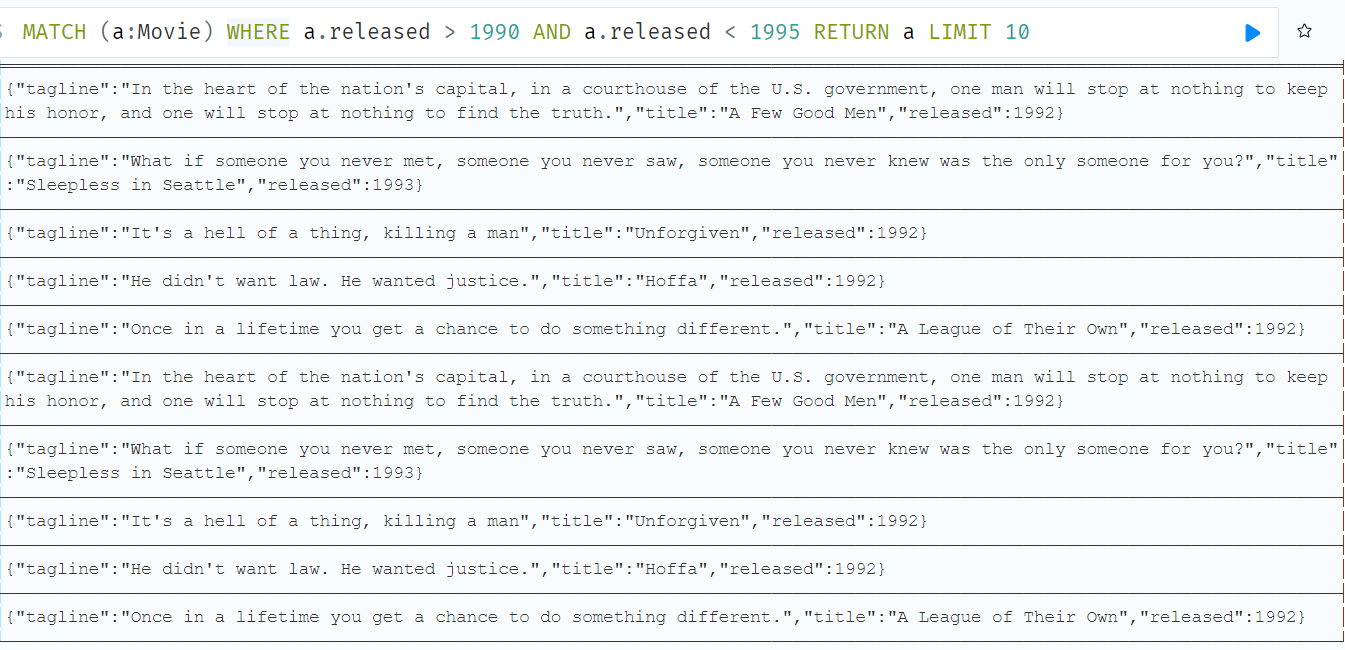
\includegraphics[scale=0.4]{Graficos/peli.png}
    \caption{Nodos película que se hayan realizado entre los años 1990 y 1995}
    \label{fig:peli}
\end{figure}
\subsubsection{Consultas complejas para evaluaciones complejas}
Para estas consultas tendremos un fin en concreto para hacer futuras relaciones.
\begin{itemize}
    \item Encontrar actores con los que cierto actor aún no haya trabajado, pero sus co-actores sí.
    En la Figura \ref{fig:coac} vemos como buscar a los coactores que no trabajaron con el actor Tom Cruise.
    \begin{figure}[H]
    \centering
    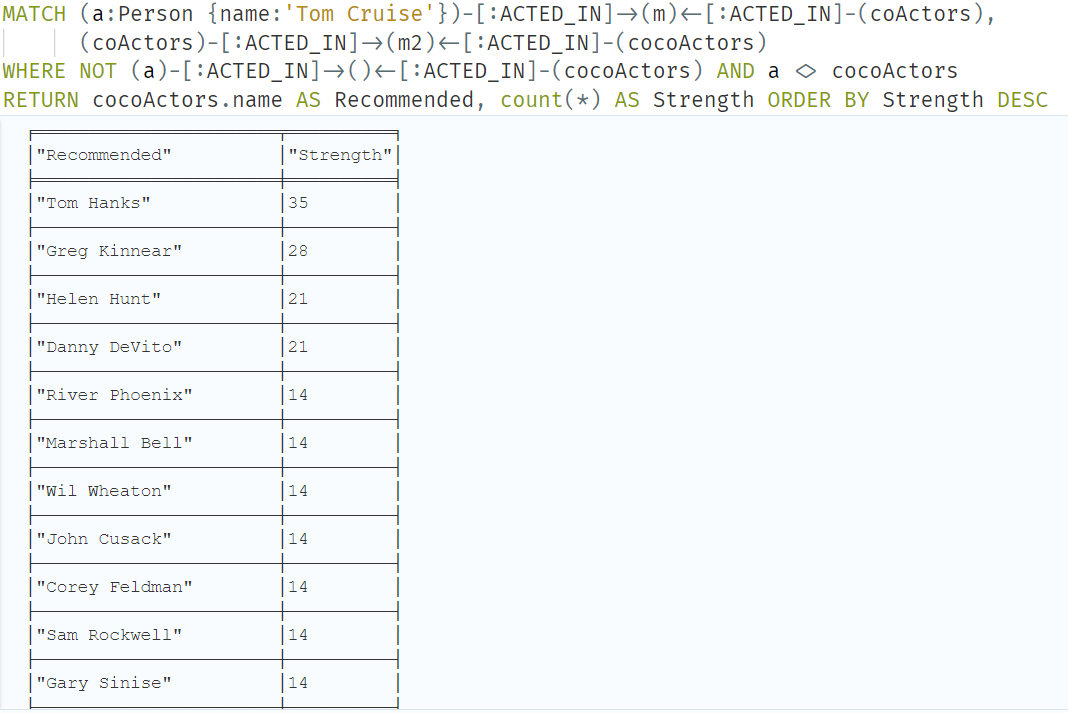
\includegraphics[scale=0.6]{Graficos/coactors.png}
    \caption{Tablero en orden descendente de la cantidad de coactores de actores principales}
    \label{fig:coac}
    \end{figure}
    \item Encontrar todas las personas que participaron en una película en concreto y que roles tuvieron en dicha película.
    En la Figura \ref{fig:inter} vemos como retornar todas las personas relacionadas a una película en concreto.
    \begin{figure}[H]
    \centering
    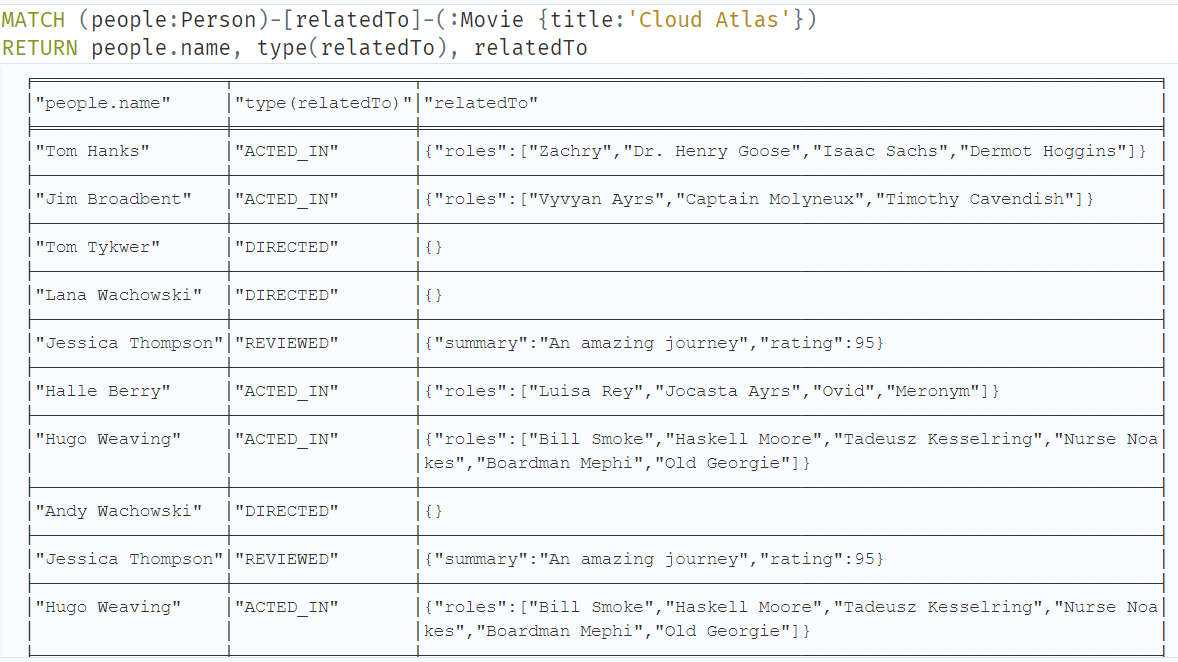
\includegraphics[scale=0.5]{Graficos/interact.png}
    \caption{Personas que interacturan en dicha película basada en las relaciones que tienen con esta.}
    \label{fig:inter}
    \end{figure}
\end{itemize}
\section{Base de datos de investigación universitaria en Neo4j}
Para los parámetros de evaluación de comparación no se tomará en cuenta el rendimiento ni la velocidad de ejecución de las consultas de dicho lenguaje, ya que, no se asegura saber que esten ejecutandose en las mismas condiciones.
Sin embargo, tomaremos en cuenta los siguientes aspectos:
\begin{itemize}
    \item Costo de la infrestructura.
    \item Velocidad de sintaxis (escritura y digitación de la misma).
    \item Comprensión del lenguaje.
    \item Facilidad de aprendizaje.
    \item Apoyo visual que sea atractivo, entendible y fácil de interpretar.
\end{itemize}
\subsection{Comparación SQL vs CYPHER Caso 1:}
La consulta de grafos escrita en Cypher es eficiente y simple. Podría decirse que puede ser formulado y realizado por trabajadores del conocimiento con menos experiencia que recibieron la formación previa y equipado con información tal como nodo y relación de nodo.
Además, la información visual que se muestra también es informativa y adecuada para diferentes niveles de espectadores, desde el conocimiento de  trabajadores a ejecutivos.\\
En la Figura \ref{fig:neo1} vemos la primera consulta en lenguaje cypher el cual consta de 1 linea de código cypher el cual realiza una unión entre resultados de búsqueda especificadas por las variables respectivas encontrando los artículos, autores y co-autores del proyecto de investigación buscado , muestra quienes interactuan de manera relacional con dicho proyecto de investigación.
Nos da la facilidad como desarrolladores o analistas de ver la cantidad de personas con sus respectivos roles y una imágen gráfica el cual representa la estructura de nodos y relaciones que involucran a dicho proyecto de investigación.\\
Una consulta más larga para responder a la misma pregunta en un relacional
La base de datos sería similar a la de la Figura \ref{fig:sql1}. La diferencia es clara. En una base de datos relacional, el requisito debe ser muy explícito por adelantado para que se traduzca correcta y cuidadosamente en consultas antes de decidir qué tablas unir en qué columnas y qué campos deben recuperarse. De hecho, requiere algunos nivel de experiencia técnica para ejecutarlo.
    \begin{figure}[H]
    \centering
    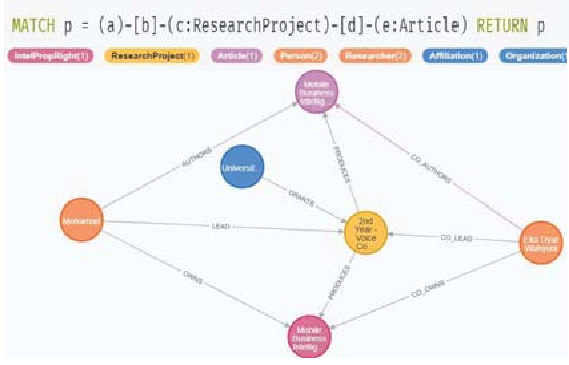
\includegraphics[scale=0.8]{Graficos/neo11.png}
    \caption{Caso 1: consulta Cypher}
    \label{fig:neo1}
    \end{figure}
    \begin{figure}[H]
    \centering
    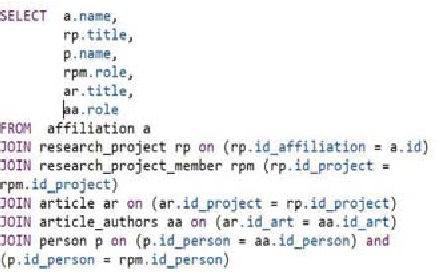
\includegraphics[scale=0.7]{Graficos/sql1.png}
    \caption{Caso 1 : Consulta SQL}
    \label{fig:sql1}
    \end{figure}+

\subsection{Comparación SQL vs CYPHER Caso 2:}
La consulta Cypher en la Figura \ref{fig:neo2} es abstracta y más natural
ya que las relaciones y los nodos subyacentes no son claramente
definido, pero solo se supone que existe. Sin embargo,los gráficos devueltos son informativos y brindan rápidamente información útil, que en una base de datos relacional es difícil de proporcionar.
Usando una base de datos relacional como se muestra en la Figura \ref{fig:sql2}, la consulta requiere pasos más largos, uniones y tiempo para ejecutarlo, especialmente cuando el tamaño de la base de datos es grande. Como la consulta anterior, es demasiado técnico y no fácilmente entendido por la gente en general y incluso trabajadores del conocimiento.

\begin{figure}[H]
    \centering
    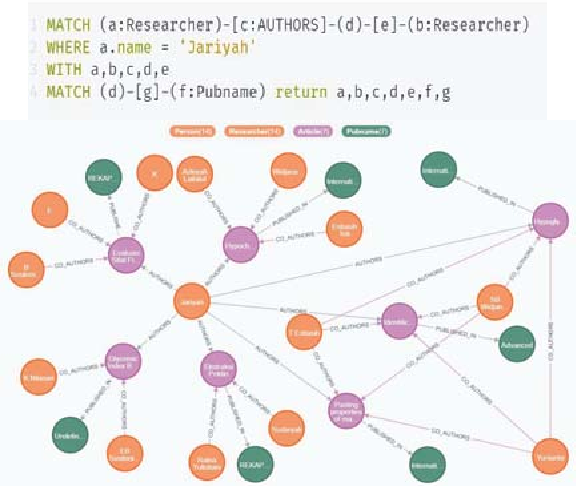
\includegraphics[scale=0.7]{Graficos/neo2.png}
    \caption{Caso 2 : Consulta Cypher}
    \label{fig:neo2}
    \end{figure}
\begin{figure}[H]
    \centering
    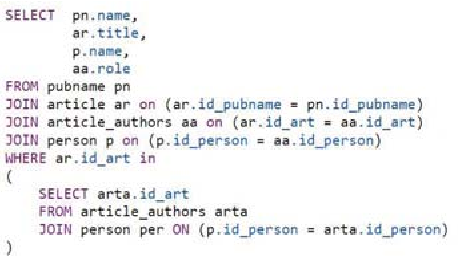
\includegraphics[scale=0.7]{Graficos/sql2.png}
    \caption{Caso 3 : Consulta SQL}
    \label{fig:sql2}
    \end{figure}
\subsection{Comparación SQL vs CYPHER Caso 3:}
Para el caso 3, la pregunta espera que exista(n) relación(es)
entre organizaciones de una forma u otra, ya sea directamente
o indirectamente. Una relación directa (a un enlace de distancia) sería algo así como Organización X HAS\_MOU\_WITH como Organización Y. Por otro lado, una conexión indirecta probablemente se manifestaría en algo como la Organización X EMPLEA a una Persona P que ESCRIBE un Artículo que es CO\_ESCRITO por una Persona P2 que TRABAJA para la Organización Y.
En este caso, hay cuatro relaciones entre Organización
X y Organización Y. La respuesta en CYPHER es tan natural
como puede ser, como se muestra en la Figura \ref{fig:neo3}.
Como se demostró en el caso 1, caso 2 y caso 3, el gráfico
la base de datos y la consulta hacen el trabajo de responder consultas
de manera eficiente en comparación con la base de datos relacional. Estos simples experimentos están en línea con estudios previos que compararon
base de datos de gráficos (neo4j) y otros sistemas de bases de datos.
Los resultados también revelan que las consultas gráficas formuladas
están muy cerca de los lenguajes naturales indicados en las consultas de perspectivas múltiples. Para directores o líderes universitarios que
a menudo se encuentran en medio de reuniones en las que se les solicita
para proporcionar información aleatoria y ad-hoc sobre su
universidades, las capacidades de las consultas gráficas sin duda serán
beneficioso.
Además de las funciones de informes y análisis compatibles
por consultas y bases de datos relacionales, que la mayoría de los ejecutivos
Los sistemas de información (EIS) que tienen actualmente, las organizaciones pueden necesitar desarrollar capacidades gráficas y analíticas respaldadas
por bases de datos gráficas y consultas.
Estudios previos por capacidades de chatbot agregadas
a la EIS existente para que los ejecutivos puedan ver y obtener
información sobre sus universidades ordenando a través de
voces y textos. Los problemas con esos sistemas son que no se sabe más allá del conocimiento específico incrustado en ellos.
Los comandos son limitados porque ellos y sus consultas SQL asociadas deben estar predefinidos primero. Entonces, esos sistemas tienen solicitudes de información aleatorias y ad hoc no atendidas.
La base de datos de gráficos y las consultas tienen grandes posibilidades de
superar ese problema. Pueden entender y producir los resultados de manera intuitiva a pesar de las preguntas a ciegas, que parecen difíciles de
comprender y parecer sin sentido, como se muestra en el Caso 1 y
Caso 2. El nodo-relación-nodo posiblemente se convertirá en el
clave en la interpretación de solicitudes aleatorias de información siempre que
podemos mapear cosas a nodos en la base de datos. De hecho, la implementación seguirá siendo un desafío, especialmente cuando se integran datos de diferentes bases de datos, a menudo sistemas heredados, donde la documentación está menos disponible o no existe.
\begin{figure}[H]
    \centering
    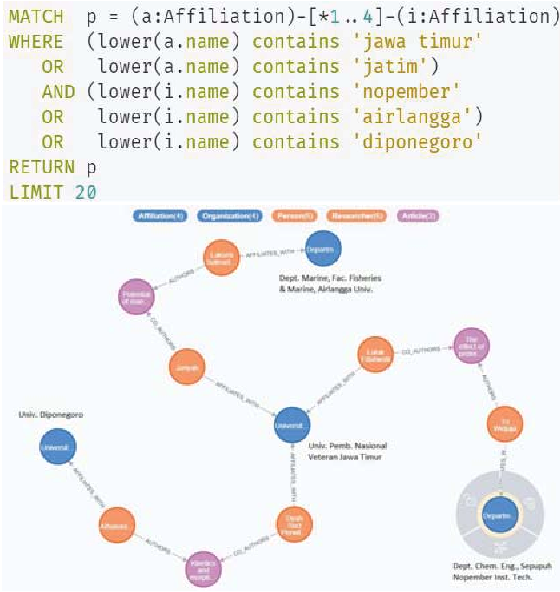
\includegraphics[scale=0.8]{Graficos/neo33.png}
    \caption{Caso 3 : Consulta Cypher}
    \label{fig:neo3}
    \end{figure}
\subsection{Ventajas que propone el Neo4j con la base de datos en lenguaje Cypher}
Al basarnos en un sistema en concreto, trabajando con una base de datos de investigadores para el respaldo de la información de los estudiantes universitarios, se detectó las siguientes ventajas:
\begin{itemize}
    \item La base de datos de gráficos de investigación presentada en este estudio tiene demostrado responder de manera eficiente a las consultas en comparación con la base de datos relacional.
    \item La base de datos de gráficos de investigación presentada en este estudio proporcionan visualmente atractivos discernimiento.
    \item La sintaxis del lengua Cypher se asemeja al lenguaje natural para la correcta interpretación de una persona con un conocimiento promedio de dicha disciplina, apoyado de un material visual que respalda dicha sintaxis.
    \item Sql es destacado por ser un lenguaje usado netamente por programadores de mucha experiencia, los cuales tienen mucho tiempo estudiando no solo el entorno de bases de datos sino también el lenguaje de SQL, como realizar transacciones y consultas correspondientes, sin embargo, se apoyan de herramientas como la ingeniería reversa para plasmar sus arquitecturas en tablas organizacionales las cuales muestran de manera robótica los nodos y relaciones.
    \item Las consultas SQL extensas no solo requieren más tiempo para ejecutarse, sino que también es más probable que incluyan errores de codificación humana debido a su complejidad. Además, las consultas más breves aumentan la facilidad de comprensión y mantenimiento en todo su equipo de desarrolladores.
    \item Cypher está diseñado para que los desarrolladores, los profesionales de bases de datos y las partes interesadas del negocio lo lean y entiendan fácilmente. Es fácil de usar porque coincide con la forma en que describimos intuitivamente los gráficos mediante diagramas.
    \item La noción básica de Cypher es que le permite pedirle a la base de datos que busque datos que coincidan con un patrón específico. Coloquialmente, podríamos pedirle a la base de datos que “encuentre cosas como esta”, y la forma en que describimos cómo se ven “cosas como esta” es dibujándolas usando arte ASCII .
    \item Un lenguaje de consulta representa su modelo de cerca. Es por eso que SQL se trata de tablas y JOIN, mientras que Cypher se trata de relaciones entre entidades. Tanto como el modelo gráfico es más natural para trabajar, también lo es Cypher, ya que toma prestado de la representación pictórica de círculos conectados con flechas que cualquier interesado (ya sea técnico o no técnico) puede entender.
    \item En una base de datos relacional, el proceso de modelado de datos se abstrae hasta ahora de las consultas SQL reales del día a día que existe una gran disparidad entre el análisis y la implementación. En otras palabras, el proceso de construcción de un modelo de base de datos relacional no es adecuado para hacer (y responder) preguntas de manera eficiente desde ese mismo modelo.
    Los modelos de bases de datos de gráficos, por otro lado, no solo comunican cómo se relacionan sus datos, sino que también lo ayudan a comunicar claramente los tipos de preguntas que desea hacer sobre su modelo de datos. Los modelos gráficos y las consultas gráficas son solo dos caras de la misma moneda.

\end{itemize}